\documentclass[12pt,brazil]{beamer}
\usepackage[utf8]{inputenc}
\usepackage[portuguese]{babel}
\setcounter{secnumdepth}{3}
\setcounter{tocdepth}{3}
\usepackage{movie15}
\usepackage{graphicx}
\setbeamercovered{transparent}
\usetheme{Boadilla}
\usepackage{times}
\usefonttheme{structurebold}
\usepackage{pgf}
\beamertemplatetransparentcovereddynamic
%\usepackage{multimedia}

\usepackage{cancel}
\usepackage{multicol}
\usepackage{multirow}
\usepackage{hyperref}


\title{Revisão de Mecânica Quântica}
\subtitle{Aula do MNPEF - Polo 41}
\author{Evy A. Salcedo Torres}
\date{\today}

\begin{document}

%%%%%%%%%%%%%%%%  SLIDE 1 %%%%%%%%%%%%%%%%%%%%%%%%%%%

\begin{frame}
  \titlepage
\end{frame}


\section{Antecedentes}

%%%%%%%%%%%%%%%%  SLIDE 2 %%%%%%%%%%%%%%%%%%%%%%%%%%%

\begin{frame}
  \frametitle{Nascimento da Espectroscopia}

  \begin{multicols}{2}
    \begin{minipage}[b][20ex][t]{\linewidth}
    \vspace*{0.5cm}
      Em 1850 Gustav Kirchhoff e Robert Bunsen analisam a luz emitida por diferentes elementos ao serem aquecidos utilizando espectrômetro inventado por Joseph Fraunhofer
    \end{minipage}

    \begin{minipage}[b][20ex][t]{\linewidth}
      \begin{figure}
        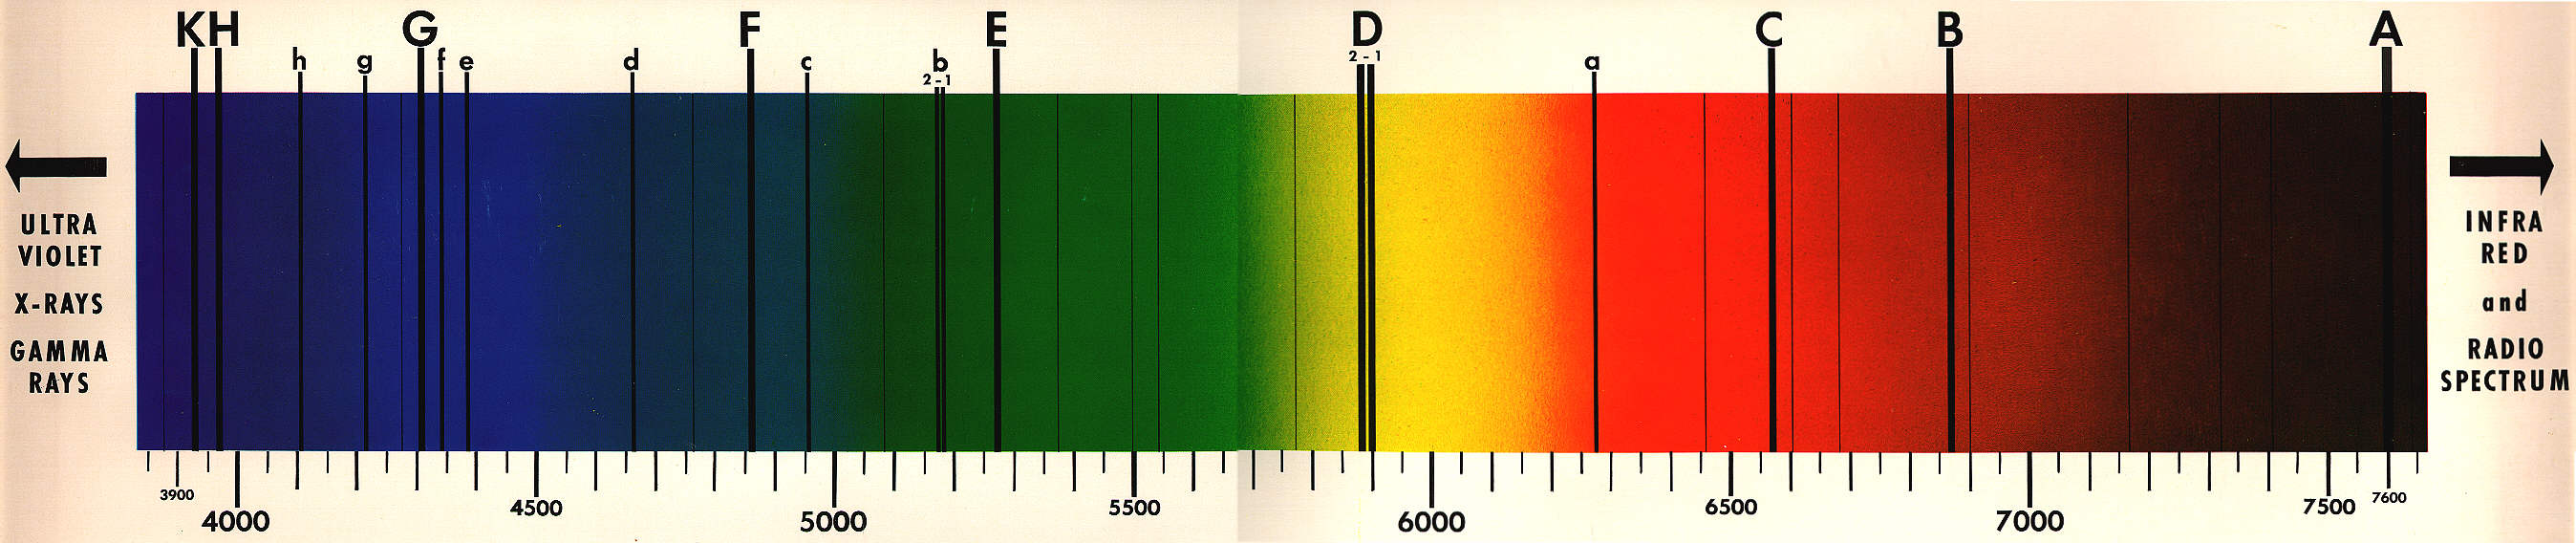
\includegraphics[width=12cm]{figuras/fig02}
      \end{figure}
    \end{minipage}

    \begin{minipage}[b][40ex][t]{\linewidth}
    \vspace*{0.5cm}
      \begin{figure}
        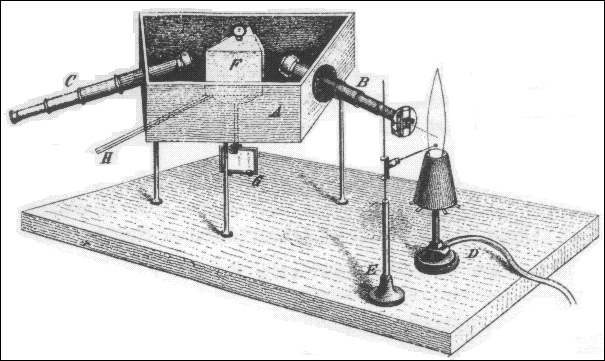
\includegraphics[width=5.5cm]{figuras/fig01}
      \end{figure}
    \end{minipage}
  \end{multicols}
\end{frame}

%%%%%%%%%%%%%%%%  SLIDE 3 %%%%%%%%%%%%%%%%%%%%%%%%%%%

\begin{frame}
  \frametitle{A proposta de  Kirchhoff}
    \begin{columns}[c]

      \column{6cm}
        \fontsize{12pt}{11pt}\selectfont
        Tendo como base seus estudos de emissão e absorção de luz, Gustav Kirchhoff argumenta que a emissão de radiação de um material se da devido ao aquecimento do seus átomos, em base a isso ele propõe
        \[
         \dfrac{e(\lambda)}{a(\lambda)} = R(\lambda , \, T)
        \]
        
        onde $e$ é o poder de emissão de um material e $a$ é o poder de absorção de um material.

      
      \column{4cm}
        \vspace*{-0.75cm}
        \begin{figure}
          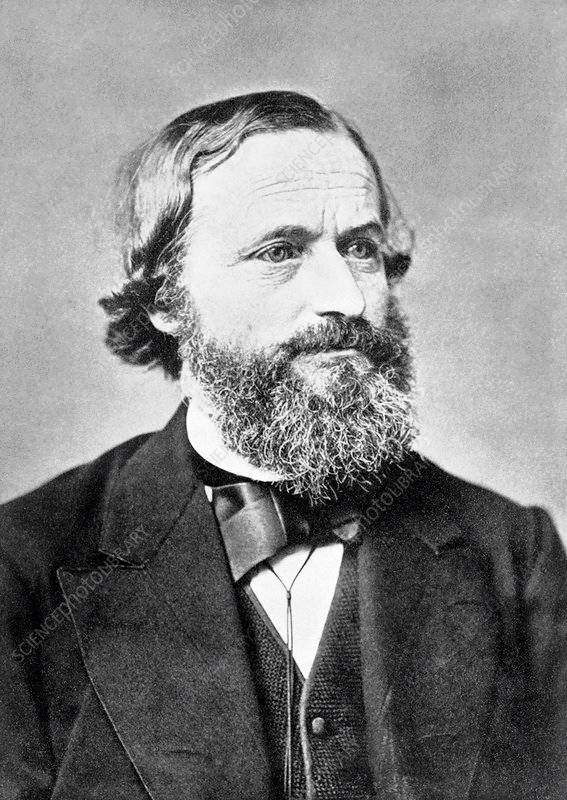
\includegraphics[width=4.5cm]{figuras/fig03}
        \end{figure}
      
    \end{columns}

\end{frame}



%%%%%%%%%%%%%%%%  SLIDE 4 %%%%%%%%%%%%%%%%%%%%%%%%%%%

\begin{frame}
  \frametitle{O corpo negro}

        \fontsize{12pt}{11pt}\selectfont
        Kirchhoff  se pergunta, como seria um corpo no qual $a=1$?, a esse corpo ideal ele chamou de corpo negro e verificaria
        \[
         e(\lambda) = R(\lambda , \, T)
        \]
        
        A proposta ideal de um corpo negro seria, uma cavidade na qual tenha um orifício sobre o qual pode incidir radiação a qual ficará atrapada dentro da cavidade e que eventualmente poderá ser emitida pelo mesmo orifício, quando o corpo entre em equilíbrio térmico com o exterior.  Dessa forma Kirchhoff abre caminho para os físicos experimentais procurarem um objeto com essa propriedade e a partir dele poderiam obter a forma funciona $f(\lambda, T)$

\end{frame}


%%%%%%%%%%%%%%%%  SLIDE 5 %%%%%%%%%%%%%%%%%%%%%%%%%%%

\begin{frame}
  \frametitle{O corpo negro}
    \begin{columns}[c]
  
    \column{5cm}
      \begin{figure}
        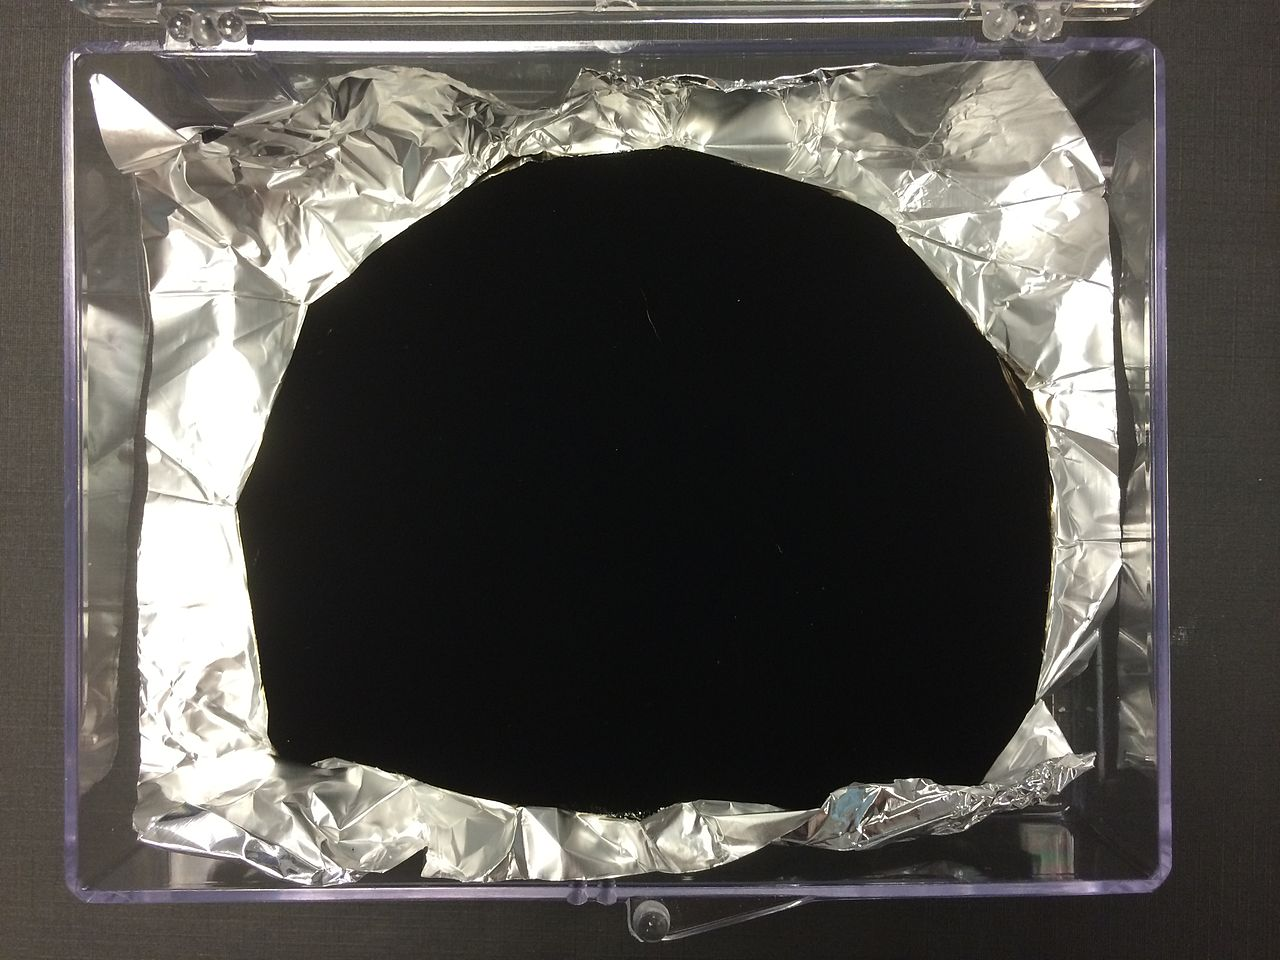
\includegraphics[width=4.5cm]{figuras/fig05}
      \end{figure}
      
    \column{5cm}
      \begin{figure}
        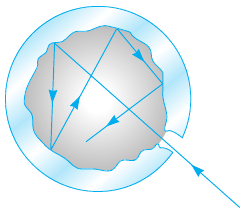
\includegraphics[width=4.5cm]{figuras/fig04}
      \end{figure}
      
    \end{columns}
    
    \href{https://www.youtube.com/watch?v=fg2x0L4YAuU}{\color{blue} Vantablack} é uma substância feita de nanotubos de carbono. É a substância mais preta conhecida, absorvendo até 99,965\% de radiação
\end{frame}



%%%%%%%%%%%%%%%%  SLIDE 6 %%%%%%%%%%%%%%%%%%%%%%%%%%%

\begin{frame}
  \frametitle{Lei de Stefan-Boltzmann}

        \fontsize{12pt}{11pt}\selectfont
        Em 1879 o físico austríaco Josef Stefan determinou experimentalmente que o fluxo de energia emitida pelo corpo negro depende da quarta potencia da temperatura, $T^4$. 
        \vspace{0.2cm}
        
        Em 1884, o também físico austríaco, Ludwig Eduard Boltzmann, utilizando argumentos termodinâmicos, obtém a chamada lei de Stefan-Boltzmann        
        \[
         P(T) = \sigma T^4
        \]
        onde $\sigma = 5,6751\times 10^{-12}\,W\,cm^2\,K^{-4}$.  

\end{frame}


%%%%%%%%%%%%%%%%  SLIDE 7 %%%%%%%%%%%%%%%%%%%%%%%%%%%

\begin{frame}
  \frametitle{Lei de Stefan-Boltzmann}
  
   \fontsize{10pt}{11pt}\selectfont
    A lei de Stefan-Boltzmann nos fornece a potência total emitida por unidade de área, que é a integral da radiância espectral $R(\lambda)$), definida tal que $R(\lambda) d\lambda$ fornece a quantidade de energia emitida pelo corpo, por unidade de tempo e de área, no intervalo de comprimentos de onda $[\lambda,\, \lambda + d\lambda]$. 
        
    \[
      P(T) = \int R(\lambda,\,T)\,d\lambda
    \]
    
    Já a densidade espectral, $\rho (\lambda, \, T)$, se relaciona com a radiância espectral via
    
    \[
      R(\lambda,\,T) = \dfrac{c}{4}\,\rho (\lambda, \, T)
    \]
    
    Por fim, a energia média se relaciona com a densidade espectral via
    
    \[
     \rho(\lambda , \, T) \, d\lambda = \bar{E}(\lambda , \, T)  n(\lambda , \, T) d\lambda
    \]
    sendo $n(\lambda , \, T)$ o número de OEM por unidade de volume, cuja comprimentos de onda esta dentro de $[\lambda,\, \lambda + d\lambda]$
    
    

\end{frame}




%%%%%%%%%%%%%%%%  SLIDE 8 %%%%%%%%%%%%%%%%%%%%%%%%%%%

\begin{frame}
  \frametitle{Lei de deslocamentos de Wien}
  
        \fontsize{10pt}{11pt}\selectfont
        A lei leva o nome de Wilhelm Wien, que formulou a relação em 1893 com base em um argumento termodinâmico. Wien considerou a expansão adiabática de uma cavidade contendo ondas de luz em equilíbrio térmico. Ele mostrou que sob expansão ou contração adiabática, a energia da luz muda exatamente da mesma maneira que a frequência. Isso significa que a frequência de pico deve mudar com a temperatura à medida que a energia passa, o que implica em 
        
        \[
          \lambda_{max} = \dfrac{b}{T}
        \]
        
        onde
        \[
          b = 2,989777\times 10^{-3} m K
        \]

\end{frame}



%%%%%%%%%%%%%%%%  SLIDE 9 %%%%%%%%%%%%%%%%%%%%%%%%%%%

\begin{frame}
  \frametitle{Lei de deslocamentos de Wien}
  
        \begin{figure}
          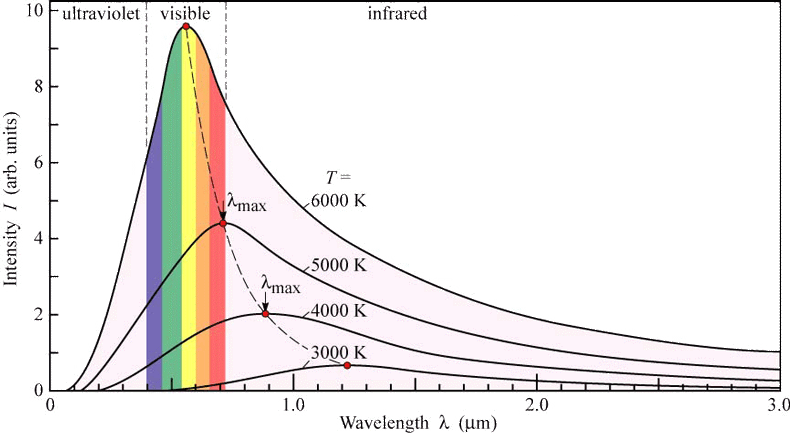
\includegraphics[width=8cm]{figuras/fig06}
        \end{figure}
        
        \[
          \lambda_{max} = \dfrac{b}{T}
        \]
  
\end{frame}


%%%%%%%%%%%%%%%%  SLIDE 10 %%%%%%%%%%%%%%%%%%%%%%%%%%%

\begin{frame}
  \frametitle{Distribuição espectral de Wien}
  
        \begin{figure}
          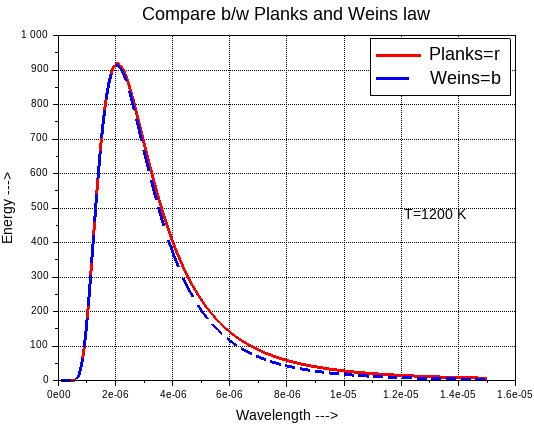
\includegraphics[width=6.cm]{figuras/fig07}
        \end{figure}
        \fontsize{10pt}{11pt}\selectfont
        
        Em 1896 Wien (Friedrich Paschen também obteve empiricamente), utilizando a teoria cinética de Boltzmann, obtém ($\alpha = 5$ nos leva a Stefan-Boltzmann se integramos em $\lambda$)
        
        \[
          \rho (\lambda, \, T)= \dfrac{c_1}{\lambda^\alpha}\exp\left(-\dfrac{c_2}{\lambda T}\right)
        \]
  
\end{frame}


%%%%%%%%%%%%%%%%  SLIDE 11 %%%%%%%%%%%%%%%%%%%%%%%%%%%

\begin{frame}
  \frametitle{Rayleigh–Jeans e a catástrofe ultravioleta}

  
  
        \begin{figure}
          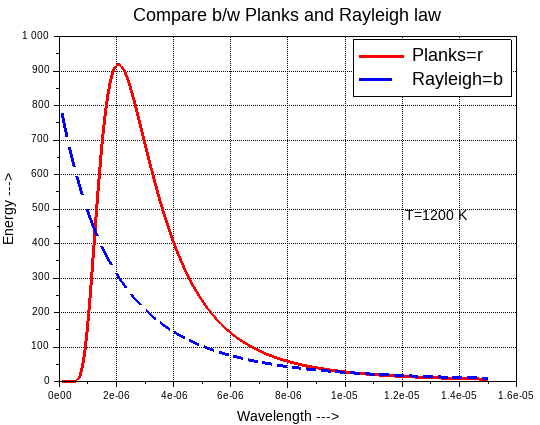
\includegraphics[width=6.cm]{figuras/fig08}
        \end{figure}
        \fontsize{9pt}{11pt}\selectfont
        
        Supondo que dentro da cavidade exite uma distribuição osciladores com energia média por modo de oscilação de $k_BT$ (teorema da equipartição), em 1900 Lord Rayleigh (ohn William Strutt) e James Jeans (1904 a versão completa)        
        \fontsize{10pt}{11pt}\selectfont
        
        \[
          \rho (\lambda, \, T) = \dfrac{8\pi k_BT}{\lambda^4}
        \]
  
\end{frame}

%%%%%%%%%%%%%%%%  SLIDE 12 %%%%%%%%%%%%%%%%%%%%%%%%%%%

\begin{frame}
  \frametitle{A lei de Planck e quantificação do campo}
  
    Para resolver o impasse Max Planck em 1900 se vê forçado a propor que a energia dos osciladores dentro da cavidade do corpo negro tem energia dada por
    \[
      E_{\nu} = nh\nu = \dfrac{nhc}{\lambda}, \quad n=1,\,2,\, 3,\, \ldots
    \]
    
    e com isso ele obtém
    
    \[
      \rho (\lambda, \, T) = \dfrac{8\pi hc }{\lambda^5\left[\exp \left(\dfrac{hc}{\lambda kT}\right) - 1\right]}
    \]
    
    com
    
    \begin{align*}    
      h &= 6,626\times 10^{-35}J\cdot s\\
        &= 4,136\times 10^{-15} eV\cdot s
    \end{align*}


\end{frame}

%%%%%%%%%%%%%%%%  SLIDE 13 %%%%%%%%%%%%%%%%%%%%%%%%%%%

\begin{frame}
  \frametitle{A lei de Planck e quantificação do campo}
  
        \begin{figure}
          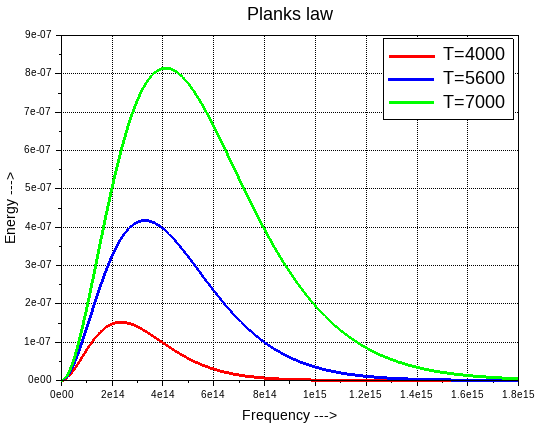
\includegraphics[width=6.5cm]{figuras/fig09}
        \end{figure}
        \fontsize{11pt}{11pt}\selectfont
  
    O, em termos da frequência
    
    \[
      \rho (\nu, \, T) = \dfrac{8\pi h \nu^3}{c^3\left[\exp \left(\dfrac{hc}{\lambda kT}\right) - 1\right]}
    \]
  
\end{frame}

%%%%%%%%%%%%%%%%  SLIDE 14 %%%%%%%%%%%%%%%%%%%%%%%%%%%

\begin{frame}
  \frametitle{Qual é a cor do Sol?}
    \begin{columns}[c]


      \column{6cm}
        \fontsize{11pt}{11pt}\selectfont
        
        O sol é branco, vemos ele amarelo porque a atmosfera dispersa o violeta, azul. O sol tem seu pico de emissão próximo do verde (se consideramos ele como sendo um corpo negro).
        \vspace*{0.5cm}

        \href{https://phet.colorado.edu/sims/html/blackbody-spectrum/latest/blackbody-spectrum_all.html}{\color{blue} Estrelas são classificadas pela sua ``cor''}
      
      \column{4cm}
        \vspace*{-0.75cm}
        \begin{figure}
          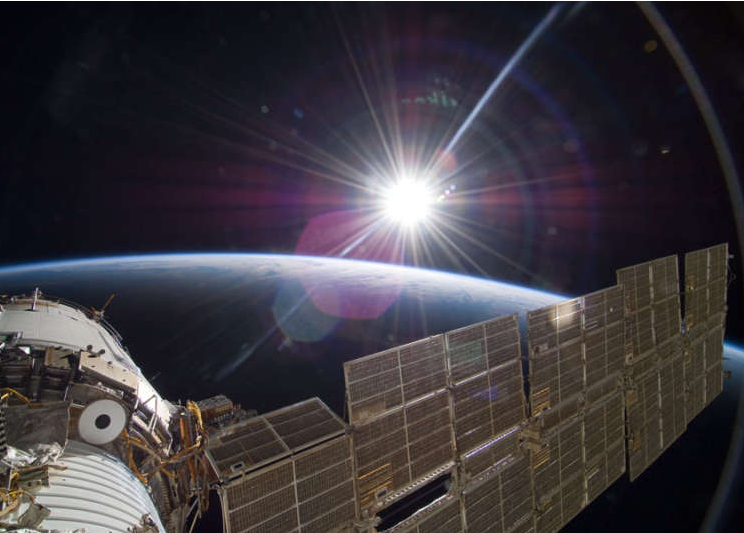
\includegraphics[width=4.5cm]{figuras/fig10}
        \end{figure}
      
    \end{columns}
  
\end{frame}


%%%%%%%%%%%%%%%%  SLIDE 15 %%%%%%%%%%%%%%%%%%%%%%%%%%%

\begin{frame}
  \frametitle{Qual é a cor do Sol?}
  
    \fontsize{11pt}{11pt}\selectfont
    
%         \vspace*{-0.75cm}
        \begin{figure}
          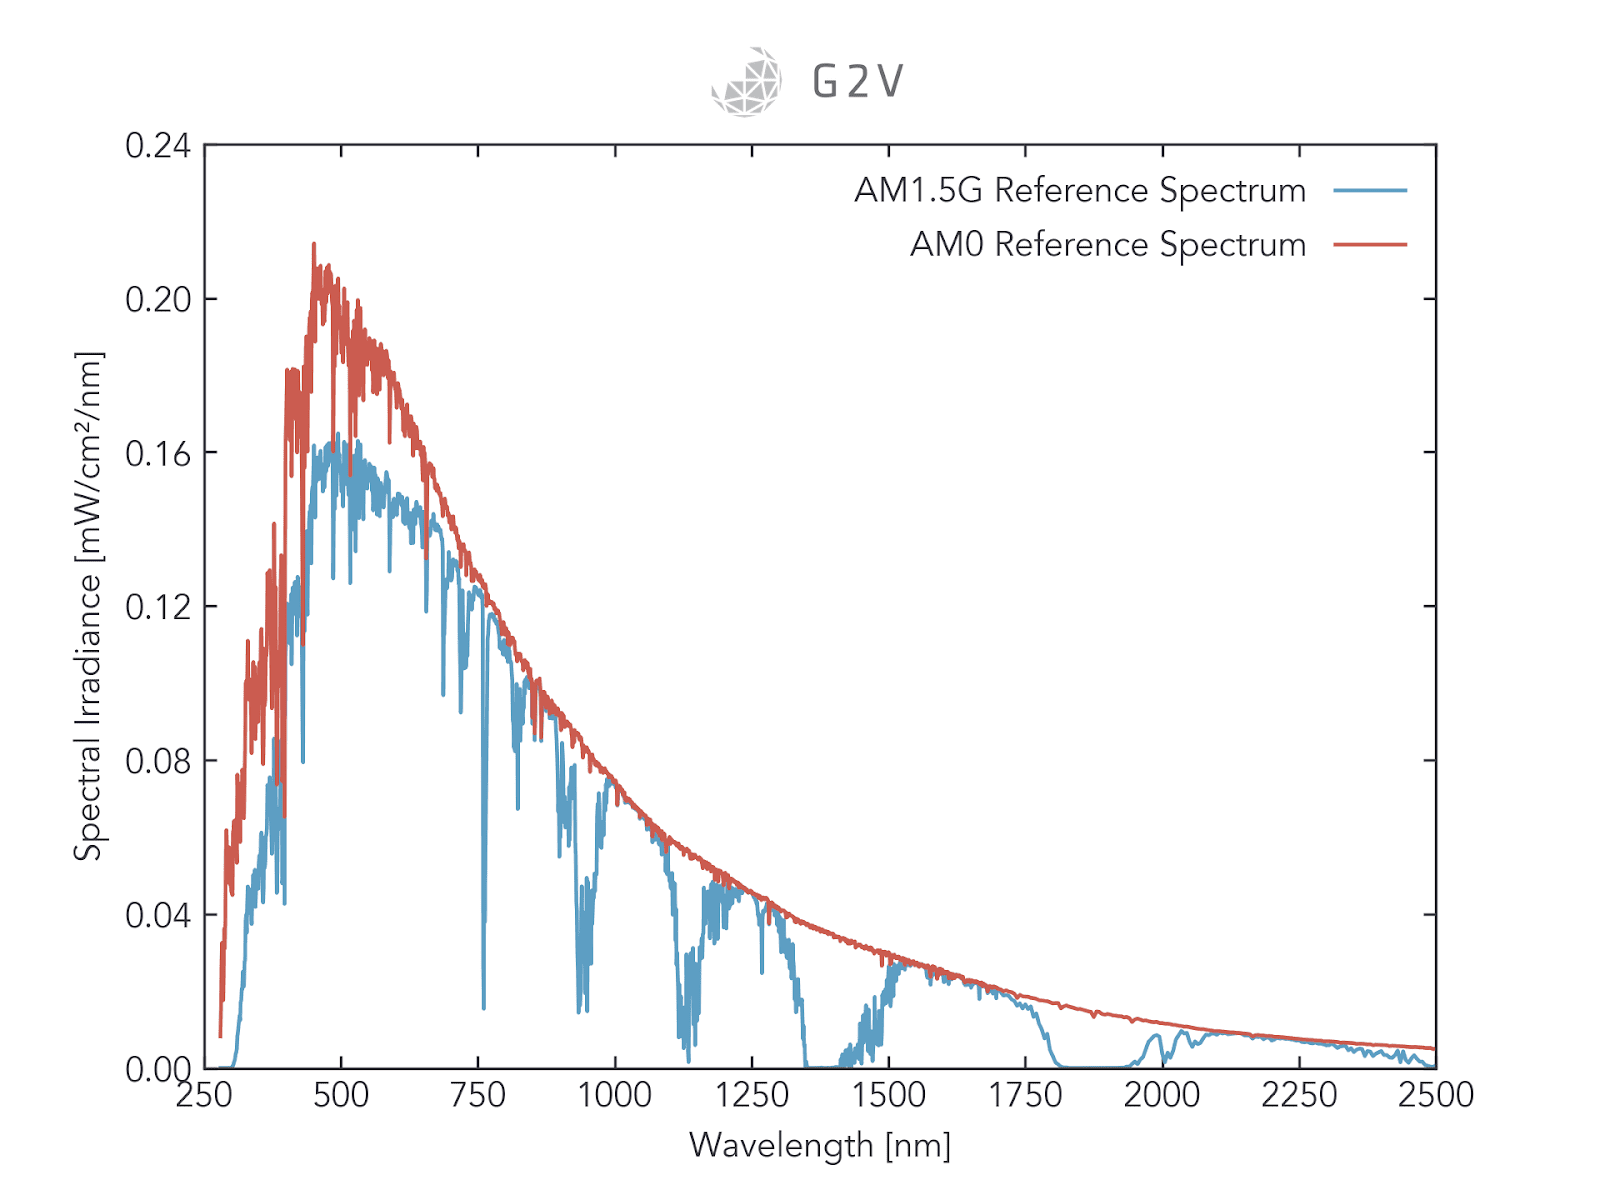
\includegraphics[width=8cm]{figuras/fig11}
        \end{figure}
      
        Espectros de referência da radiação solar. O AM indica a quantidade de ar que atravessou a luz antes de ser coletada, assim AM0 indica que é no espaço exterior, AM1 indica que atravessou 9km, e AM1.5 são 13,5 km
    
\end{frame}



%%%%%%%%%%%%%%%%  SLIDE 16 %%%%%%%%%%%%%%%%%%%%%%%%%%%

\begin{frame}
  \frametitle{Fotons}
  
    \begin{columns}[c]


      \column{6cm}
        \fontsize{11pt}{11pt}\selectfont
        
        Entre 1886 e 1889 Heinrich Rudolf Hertz realiza vários experimento para verifica a existência das OEM. Num desses experimentos Hertz notou que a emissão da faísca era facilitada se um dos terminais do emissor fosse iluminado com luz ultravioleta. 
        \vspace*{0.5cm}

        \href{https://youtu.be/9gDFll6Ge7g?t=121}{\color{blue} Experimento caseiro de Hertz}
        \vspace*{0.5cm}
        
        \href{https://youtu.be/SnKKj2bonAI?t=658}{\color{blue} Experimento de Hertz com mais potência}
      
      \column{4cm}
        \vspace*{-2.5cm}
        \begin{figure}
          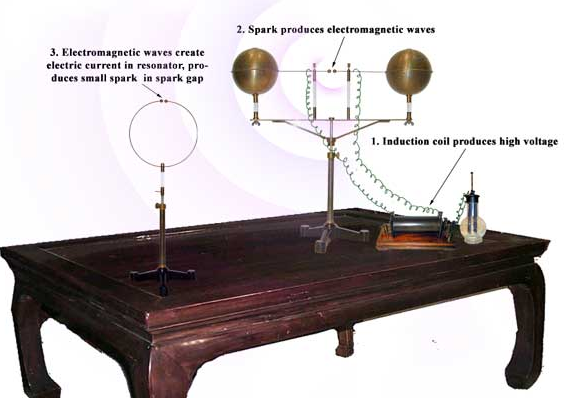
\includegraphics[width=4.5cm]{figuras/fig12}
        \end{figure}
      
    \end{columns}  
    
\end{frame}


%%%%%%%%%%%%%%%%  SLIDE 17 %%%%%%%%%%%%%%%%%%%%%%%%%%%

\begin{frame}


        \begin{figure}
          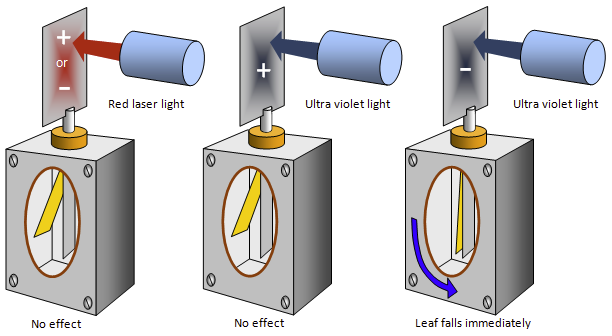
\includegraphics[width=8cm]{figuras/fig13}
        \end{figure}
        \fontsize{10pt}{11pt}\selectfont

  Em 1888 Wilhelm Hallawchs, ajudante de Hertz, decide analisar com um pouco mais de atenção o efeito da luz azul menosprezada por Hertz. Inicialmente Hallawchs carrega negativamente o eletroscópio, como consequência desse fato as placas metálicas se separam, ele observa que lentamente as placas metálicas se aproximam o que indica que a carga negativa está diminuindo (ou aumentando a carga positiva). Quando ele fazia incidir luz ultravioleta sobre o polo do eletrodo as placas se uniam abruptamente, o que indicava que o eletroscópio subitamente deixau de ter carga negativas em excesso.

\end{frame}


%%%%%%%%%%%%%%%%  SLIDE 18 %%%%%%%%%%%%%%%%%%%%%%%%%%%

\begin{frame}
  \frametitle{Fotons - Experimento de Lennard}

  \begin{figure}
          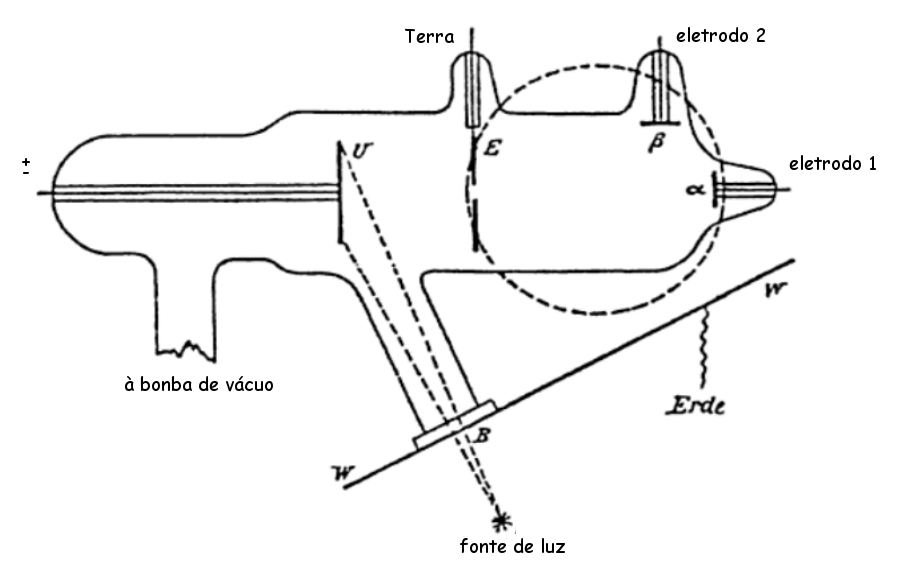
\includegraphics[width=8cm]{figuras/fig14}
  \end{figure}
  
  Montagem experimental de Phillip Lenard de 1902

\end{frame}


%%%%%%%%%%%%%%%%  SLIDE 19 %%%%%%%%%%%%%%%%%%%%%%%%%%%

\begin{frame}
  \frametitle{Fotons - Experimento de Lennard}
        \fontsize{11pt}{11pt}\selectfont
  
        \vspace*{-0.5cm}
  \begin{enumerate}
   \item A energia dos elétrons individuais emitidos independem da intensidade da radiação utilizada
   \item A intensidade da radiação resulta num incremento no número de elétrons.
   \item A energia de elétrons individuais depende da cor da luz utilizada, menor comprimento de onda implica em maior energia dos elétrons. 
  \end{enumerate}
        \vspace*{0.5cm}
  
  Também observou que existia um valor limite de energia com que os elétrons eram expelidos, já que o potencial do ânodo, $U'$ na figura, era controlado

        \vspace*{0.5cm}
  
        \href{https://phet.colorado.edu/sims/cheerpj/photoelectric/latest/photoelectric.html?simulation=photoelectric&locale=pt}{\color{blue} Simulação PHET}
\end{frame}


%%%%%%%%%%%%%%%%  SLIDE 20 %%%%%%%%%%%%%%%%%%%%%%%%%%%

\begin{frame}
  \frametitle{Teoria quântica de Einstein para o efeito fotoelétrico}
        \fontsize{11pt}{11pt}\selectfont
  
        \vspace*{-0.5cm}
  \begin{enumerate}
   \item A luz é emitida da mesma forma como é feita pelos osciladores da cavidade do corpo negro, em pacotes localizados de radiação com energia dada pela relação de Planck, $E=h\nu$
   \item Os pacotes de radiação não se dispersam quando se deslocam da fonte de luz até o eletrodo, assim eles se movem de forma localizada, similarmente a como se desloca uma partícula.
   \item Cada pacote de radiação que atinge a superfície do eletrodo deposita toda sua energia $h\nu$ num único elétron da superfície. 
  \end{enumerate}
\end{frame}


%%%%%%%%%%%%%%%%  SLIDE 21 %%%%%%%%%%%%%%%%%%%%%%%%%%%

\begin{frame}
  \frametitle{Teoria quântica de Einstein para o efeito fotoelétrico}

  \begin{multicols}{2}
    \begin{minipage}[b][20ex][t]{\linewidth}
    \vspace*{0.25cm}
      \begin{figure}
        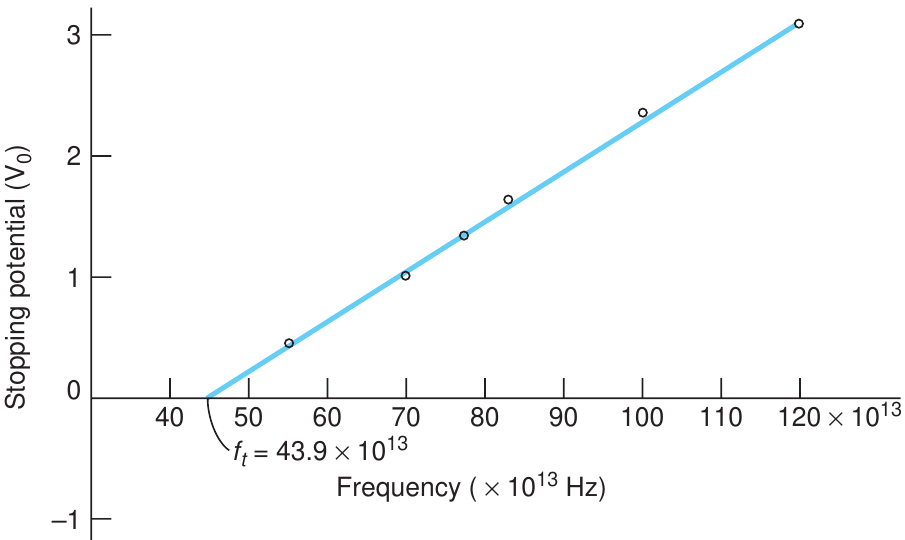
\includegraphics[width=6.0cm]{figuras/fig16}
      \end{figure}
      \fontsize{8pt}{11pt}\selectfont
      Resultado obtido por Millikan em conformidade com Einstein, $V_0$ função linear de $\nu$
    \end{minipage}

    \begin{minipage}[b][20ex][t]{\linewidth}    
    \vspace*{1.25cm}
      \[
       eV_0 = h\nu - \phi
      \]
    \end{minipage}

    \begin{minipage}[b][40ex][t]{\linewidth}
    \vspace*{-1cm}
      \begin{figure}
        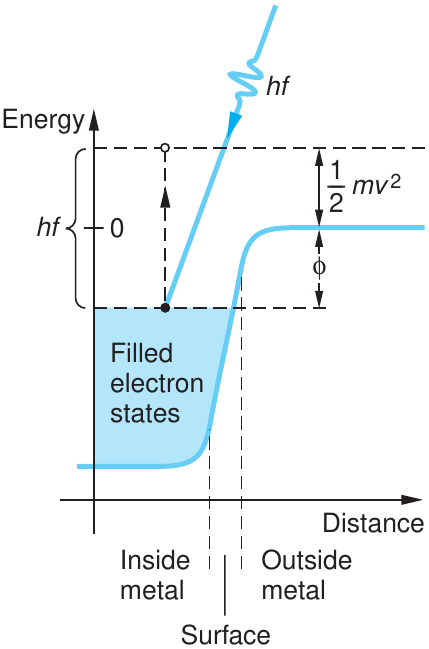
\includegraphics[width=5.cm]{figuras/fig15}
      \end{figure}
      
    \end{minipage}
  \end{multicols} 

\end{frame}


%%%%%%%%%%%%%%%%  SLIDE 22 %%%%%%%%%%%%%%%%%%%%%%%%%%%

\begin{frame}
  \frametitle{Efeito fotoelétrico inverso}
    \begin{columns}[c]


      \column{6cm}        
      \fontsize{8pt}{11pt}\selectfont
      
      Conversão de energia cinética do elétron em um fóton. Como $K_e >> \phi$
      \begin{align*}
        K_e &= h\nu - \cancelto{0}{\phi}\\
        Ve &= \dfrac{hc}{\lambda}\\
        \lambda_{min} &= \dfrac{hc/e}{V}\\
        &= \dfrac{1,24\times 10^3\, nm}{V}        
      \end{align*}
      
      que é a regra de Duane-Hunt.
      
      \column{4cm}
        \vspace*{-0.75cm}
        \begin{figure}
          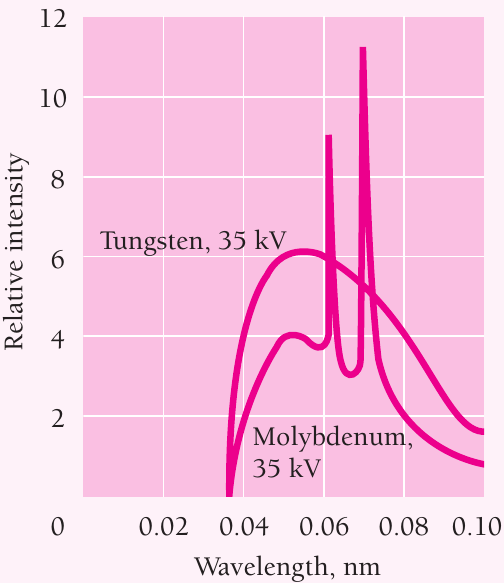
\includegraphics[width=4.5cm]{figuras/fig17}
        \end{figure}
    \end{columns}  

\end{frame}

%%%%%%%%%%%%%%%%  SLIDE 23 %%%%%%%%%%%%%%%%%%%%%%%%%%%

\begin{frame}
  \frametitle{Efeito Compton}
        \vspace*{-0.75cm}
        \begin{figure}
          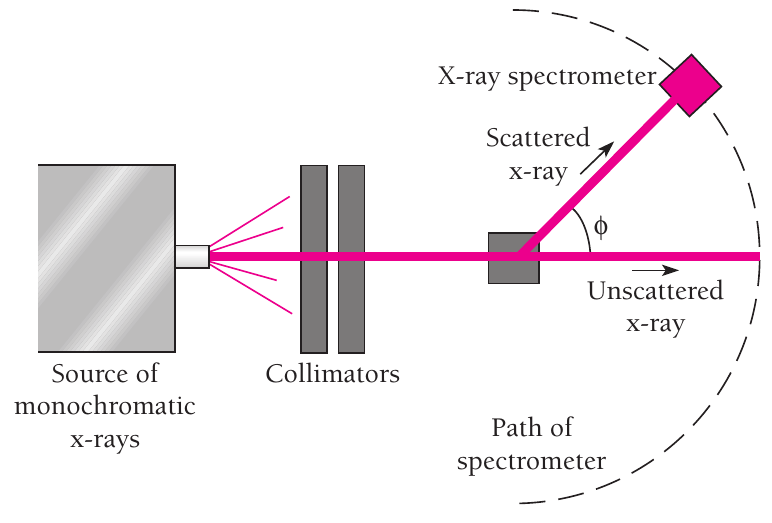
\includegraphics[width=8cm]{figuras/fig18}
        \end{figure}
        
      \fontsize{10pt}{11pt}\selectfont
        Quando raios X são difratados por uma amostra se observam dois picos, um com o comprimento de onda quase igual ao comprimento de onda original do raio X e outro com um comprimento de onda maior.

\end{frame}

%%%%%%%%%%%%%%%%  SLIDE 24 %%%%%%%%%%%%%%%%%%%%%%%%%%%

\begin{frame}
  \frametitle{Efeito Compton}
%         \vspace*{-0.75cm}
        \begin{figure}
          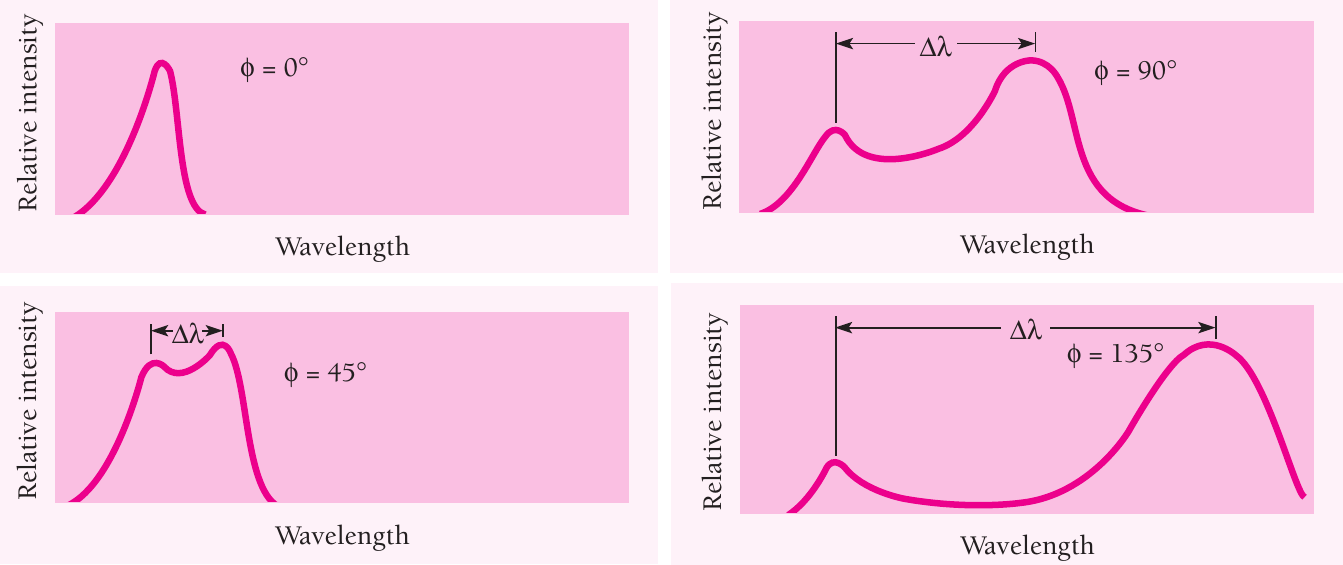
\includegraphics[width=12cm]{figuras/fig19}
        \end{figure}

\end{frame}

%%%%%%%%%%%%%%%%  SLIDE 25 %%%%%%%%%%%%%%%%%%%%%%%%%%%

\begin{frame}
  \frametitle{Efeito Compton}
        \vspace*{-0.75cm}
        \begin{figure}
          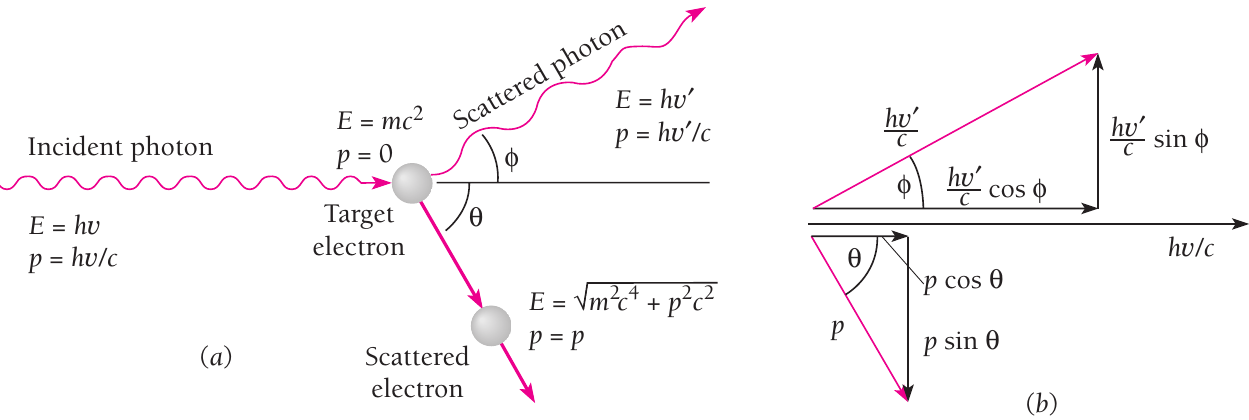
\includegraphics[width=12cm]{figuras/fig20}
        \end{figure}
        
      \fontsize{10pt}{11pt}\selectfont
        Compton considerou os fótons do raio X como sendo um partículas que colidem com o os elétron fracamente ligado (massa do elétron) e com os fortemente ligados (massa do átomo), aplicando conservação do momento obtem
        \[
         \Delta \lambda = \dfrac{h}{mc}\left(  1 - \cos \theta \right)
        \]


\end{frame}

%%%%%%%%%%%%%%%%  SLIDE 26 %%%%%%%%%%%%%%%%%%%%%%%%%%%

\begin{frame}
  \frametitle{Produção de Pares}
  

  \begin{multicols}{2}
    \begin{minipage}[b][20ex][t]{\linewidth}
    \vspace*{0.25cm}
      \begin{figure}
        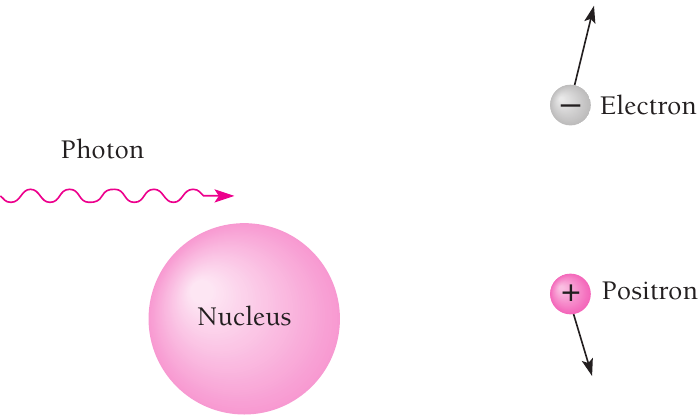
\includegraphics[width=6.0cm]{figuras/fig21}
      \end{figure}
    \end{minipage}

    \begin{minipage}[b][20ex][t]{\linewidth}    
    \vspace*{-0.5cm}
      \begin{figure}
        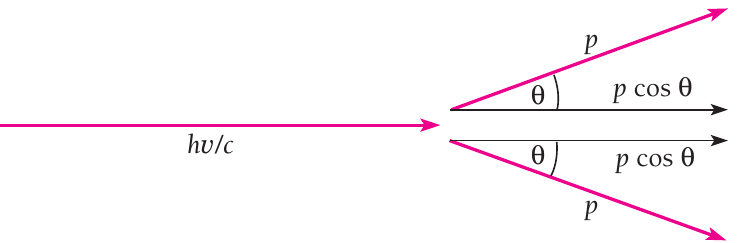
\includegraphics[width=6.5cm]{figuras/fig23}
      \end{figure}
      \fontsize{8pt}{11pt}\selectfont
      
    \end{minipage}

    \begin{minipage}[b][40ex][t]{\linewidth}
    
      \begin{figure}
        \hspace*{.5cm}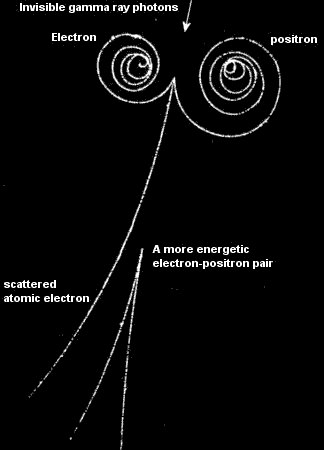
\includegraphics[width=4.5cm]{figuras/fig22}
      \end{figure}
      
    \end{minipage}
  \end{multicols} 
  
\end{frame}

%%%%%%%%%%%%%%%%  SLIDE 27 %%%%%%%%%%%%%%%%%%%%%%%%%%%

\begin{frame}
  \frametitle{O fóton como partícula}
  

  \begin{multicols}{2}
    \begin{minipage}[b][20ex][t]{\linewidth}
    \vspace*{0.25cm}
      \begin{figure}
        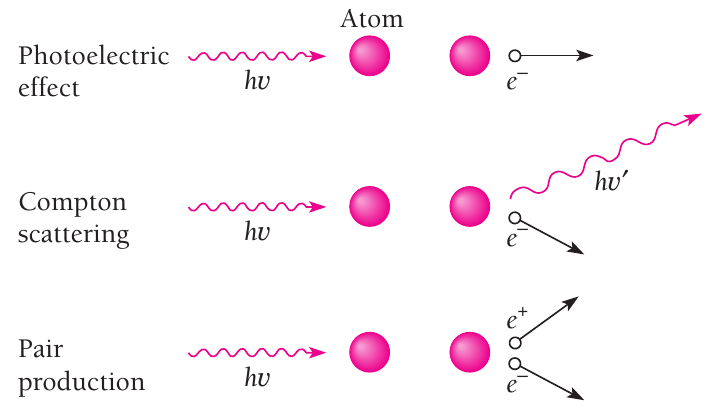
\includegraphics[width=5.0cm]{figuras/fig24}
      \end{figure}
    \end{minipage}

    \begin{minipage}[b][20ex][t]{\linewidth}    
    \vspace*{-1cm}
      \begin{figure}
        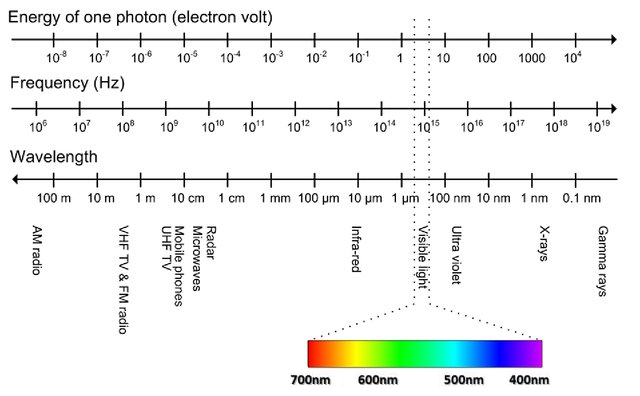
\includegraphics[width=6.5cm]{figuras/fig26}
      \end{figure}
      \fontsize{8pt}{11pt}\selectfont
      
    \end{minipage}

    \begin{minipage}[b][40ex][t]{\linewidth}    
    \vspace*{0.5cm}
      \begin{figure}
        \hspace*{.5cm}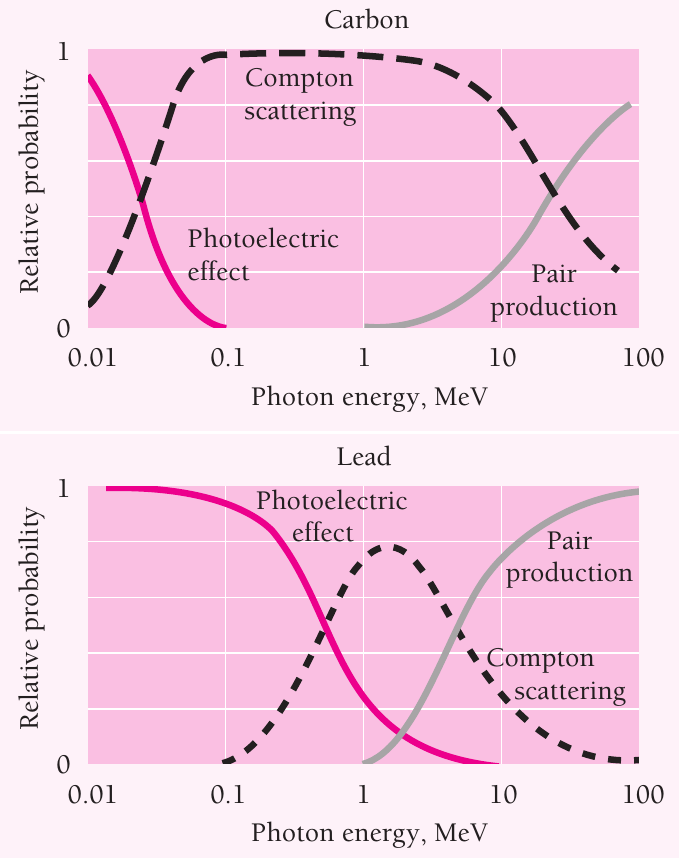
\includegraphics[width=5cm]{figuras/fig25}
      \end{figure}
      
    \end{minipage}
  \end{multicols} 
  
\end{frame}


%%%%%%%%%%%%%%%%  SLIDE 28 %%%%%%%%%%%%%%%%%%%%%%%%%%%

\begin{frame}
  \frametitle{Coeficiente de atenuação linear}
    \begin{columns}[c]


      \column{5cm}        
      \fontsize{8pt}{11pt}\selectfont
      
      A fração de energia $-dI/I$ perdida por um feixe de fótons ao passar através de uma largura $dx$ de um absorvedor é dada por
      \[
       -\dfrac{dI}{I} = \mu dx
      \]
      onde $\mu$ é o coeficiente de atenuação linear.  Integrando
      
      \[
        I = I_0 e^{-\mu x}
      \]
      
      \column{5cm}
        \vspace*{-1cm}
        \begin{figure}
          \hspace*{-.5cm}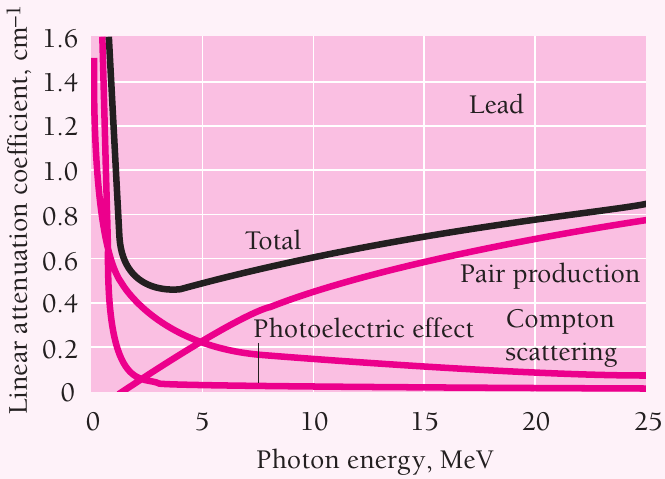
\includegraphics[width=6cm]{figuras/fig27}
        \end{figure}
    \end{columns}  

\end{frame}

%%%%%%%%%%%%%%%%  SLIDE 29 %%%%%%%%%%%%%%%%%%%%%%%%%%%

\begin{frame}
  \frametitle{Fótons caindo na Terra}
    \begin{columns}[c]


      \column{5cm}        
      \fontsize{10pt}{11pt}\selectfont
        \vspace*{-1.25cm}
      
      \begin{align*}
         E_f + mgH &= E_i\\
         h\nu' &= \left(\dfrac{h\nu}{c^2}\right)gH + h\nu\\
         h\nu' &= h\nu \left(1 + \dfrac{gH}{c^2}\right)\\
         \nu' &= \nu \left(1 + \dfrac{gH}{c^2}\right)
      \end{align*}

      
      \column{5cm}
        \vspace*{-1.cm}
        \begin{figure}          
      \hspace*{-0.5cm}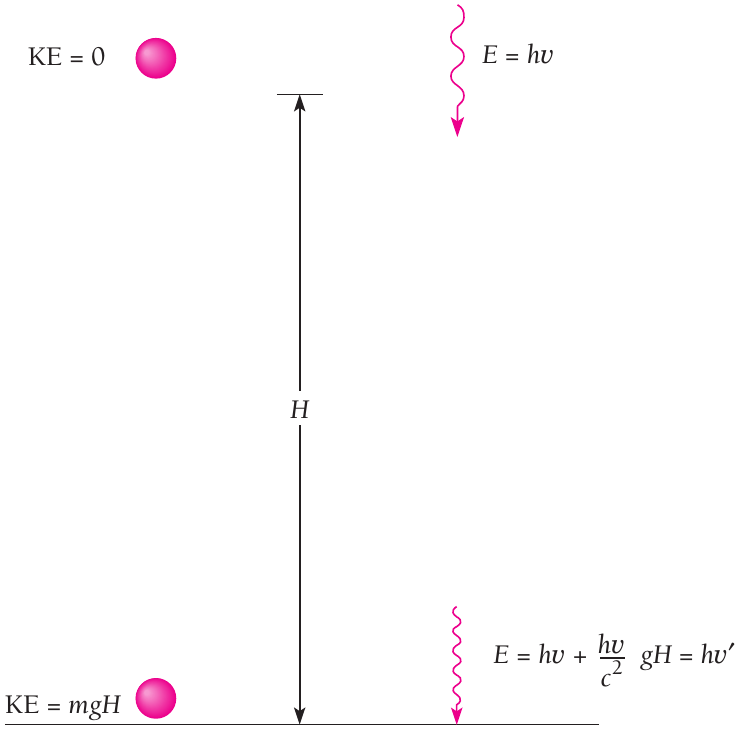
\includegraphics[width=6cm]{figuras/fig28}
        \end{figure}
    \end{columns}  

\end{frame}

%%%%%%%%%%%%%%%%  SLIDE 29 %%%%%%%%%%%%%%%%%%%%%%%%%%%

\begin{frame}
  \frametitle{O fóton escapando de Estrelas}
  

  \begin{multicols}{2}
    \begin{minipage}[b][20ex][t]{\linewidth}
    \fontsize{10pt}{11pt}\selectfont
      \begin{align*}
         E_i &= E_f - \dfrac{GMm}{R}\\
         h\nu' &= h\nu - \left(\dfrac{GM}{R}\right)\left(\dfrac{h\nu}{c^2}\right)\\
         h\nu' &= h\nu \left(1 - \dfrac{GM}{c^2R}\right)\\
         \nu' &= \nu \left(1 - \dfrac{GM}{c^2R}\right)
      \end{align*}
    \end{minipage}

    \begin{minipage}[b][20ex][t]{\linewidth}    
    \vspace*{0.5cm}
      \begin{figure}        
      \hspace*{1cm}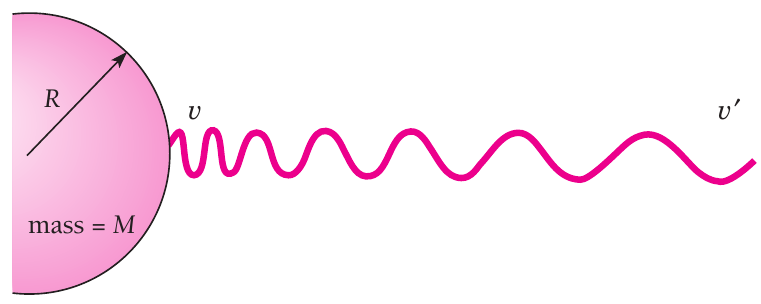
\includegraphics[width=6.5cm]{figuras/fig29}
      \end{figure}
      \fontsize{8pt}{11pt}\selectfont
      
    \end{minipage}

    \begin{minipage}[b][40ex][t]{\linewidth}    
    \vspace*{0.5cm}
      \fontsize{10pt}{11pt}\selectfont
      Classicamente, se $GM/c^2R\geq 1$ a luz não escapa da estrela, então teríamos um buraco Negro.
      \vspace*{0.25cm}
      Relatividade Geral muda para o critério para $GM/c^2R\geq 1/2$.
      
      \vspace*{0.25cm}
      O critério clássico coincide com o chamado raio de Schwarzschild, que define o horizonte de evento
      
      
    \end{minipage}
  \end{multicols} 
  
\end{frame}




\end{document}
